\section{Risultati}

In questa sezione vengono illustrati e documentati i risultati ottenuti mediante questo procedimento. 

I test sono stati effettuati considerando l'intero dataset di immagini e utilizzando la tecnica della classificazione con \emph{cross-validazione}. La cross-validazione (\emph{cross-validation} in inglese) è una tecnica statistica che consiste nel suddividere in $k$ parti equinumerose il dataset, \emph{$k$-fold cross-validation}, e, ad ogni passo, la parte $\frac{1}{k}$-esima del dataset viene ad essere il validation dataset, mentre la restante parte costituisce il training dataset. 

Così, per ognuna delle $k$ parti (in questo caso $k = 8$) si allena il modello, evitando quindi problemi di \emph{overfitting}, ma anche di campionamento asimmetrico del training dataset, tipico della suddivisione del dataset in due sole parti (ovvero training e validation dataset). In altre parole, si suddivide il campione osservato in gruppi di egual numerosità, si esclude iterativamente un gruppo alla volta e lo si cerca di predire con i gruppi non esclusi. Ciò al fine di verificare la bontà del modello di predizione utilizzato.

Una volta costruito il modello tramite questa tecnica, ne viene valutata l'efficacia: tutto il dataset viene valutato e si ottengono così i risultati di corretta o errata classificazione.

Il valore di $K$ per la creazione del modello a mistura di gaussiane scelto è 16, valore con cui è stato ottenuto il punteggio più alto di accuratezza finale.

Nella Tabella 1 vengono raccolti i dati ottenuti dalla valutazione del dataset tramite il modello.

\begin{table}[H]
\centering
\footnotesize
\begin{tabular}{|l | c | c | c |} 
 \hline 
 \textbf{Classe} &  \textbf{Totale} & \textbf{Corretti} & \textbf{Percentuale} \\ [0.5ex] 
 \hline\hline
 Punteggiato & 49 & 38 & 77.55\\
 Nucleolare & 11 & 1 & 9.09\\
 Citoplasmico & 15 & 10 & 66.67\\
 Negativo & 33 & 30 & 90.91\\
 Omogeneo & 20 & 12 & 60.00\\
 Granulare & 9 & 2 & 22.22\\
 \hline
\end{tabular}
\caption{Risultati}
\label{table:1}
\end{table}

\begin{figure}[H] 
  \centering
    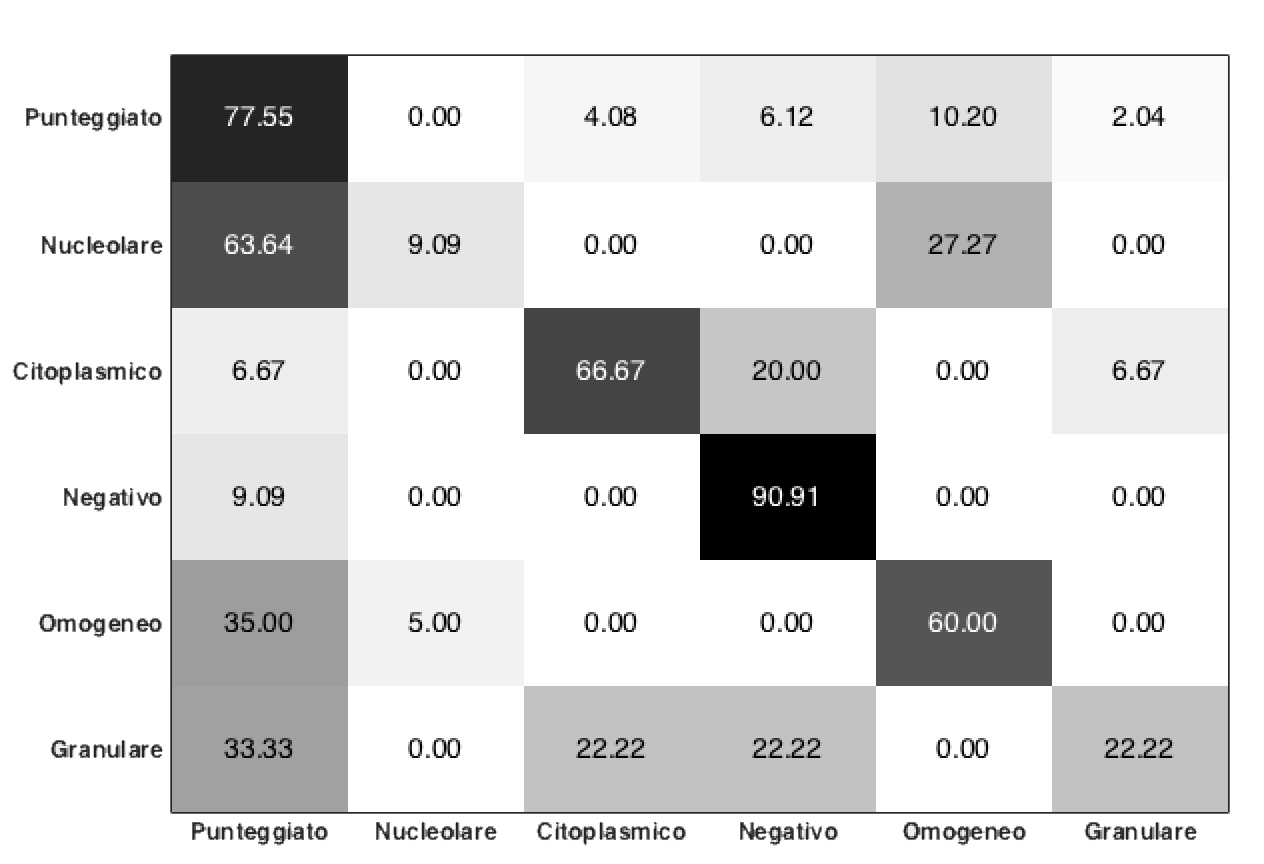
\includegraphics[width=0.9\textwidth]{images/confusion_matrix.png}
    \caption{{\small \textit{Matrice di confusione}}}
\end{figure}

Il miglior risultato ottenuto ha classificato correttamente 93 scansioni su 137, con un accuratezza totale del 67.88 \%.

Da una prima analisi sui risultati ottenuti si evince che il pattern \emph{punteggiato} è quello che ha migliore probabilità di essere correttamente classificato. Questo può dipendere anche dal fatto che è la classe con il maggior numero di esemplari e dunque il modello costruito è tendenzialmente più preciso.

Un ottimo risultato si ottiene anche per quanto riguarda il pattern \emph{negativo} che corrisponde a quelle cellule dove il marcatore fluorescente non emette luce visibile. 

I pattern \emph{nucleolare} e \emph{granulare} sono quelli che hanno ottenuto risultati peggiori. Il \emph{nucleolare}, ad esempio, viene riconosciuto correttamente una volta soltanto, confondendolo
in buona parte con il \emph{punteggiato} o con l'\emph{omogeneo}, mentre il pattern \emph{granulare} viene confuso quasi in modo equo fra tutte le altre classi. Questo può in parte dipendere da un minor numero di campioni su cui creare il modello ma anche da una varietà di cellule all'interno della stessa classe.